% Working template, NOT a completed or accepted paper. Compile with XeLaTeX.
\documentclass[UTF8,11pt]{ctexart}
\usepackage[a4paper,margin=2.4cm]{geometry}
\usepackage{amsmath,amssymb,booktabs,graphicx,hyperref}
\title{视频与毫米波人体姿态融合的几何表示与公平对照研究\\（论文工作模板）}
\author{作者及单位由接手人填写}
\date{研究快照：2026年10月16日}
\begin{document}
\maketitle
\begin{abstract}
待方法与论文主张确定后撰写。现有完整开发证据不支持几何自由残差全面优于同观测神经网络；最终保留集未评价。不要将此模板当作完成稿。
\end{abstract}
\section{引言}
明确研究问题、应用范围与评价对象。mRI与X-Fi为相关公开研究\cite{an2022mri,chen2025xfi}。
\section{相关工作}
讨论相机几何与雷达定位先例\cite{knap2024lifting,amin2023radar}，逐篇区分全文、摘要和题录核验程度。
\section{方法}
从handoff交接说明和原源码转写坐标约定、训练内深度拟合、主体OOF、门控及自由残差。标准透视、OOF和残差学习不单独宣称原创。
\section{数据与实验协议}
16开发主体，12288帧；12训练主体9216帧，4验证主体3072帧；一个划分、三个初始化。保留3/10/12/18未评价。明确异常标签、筛查敏感性和合成图像退化。
\section{结果与消融}
完整主表取自large\_protocol\_all\_methods.csv，不从正文手工挑数。几何自由残差与同观测MLP的正常误差为60.2021和60.1238mm，综合S为81.5609和81.4391mm；GRU的综合S为79.7126mm。需保留这些负结果。
\begin{figure}[htbp]\centering
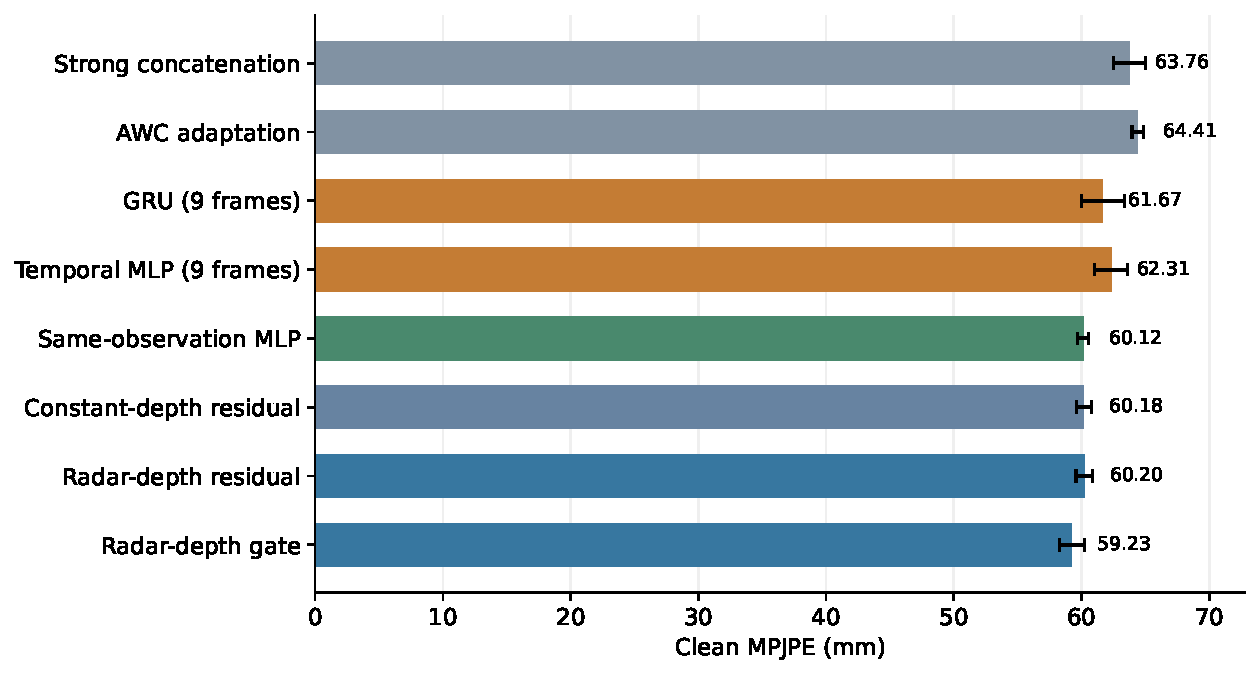
\includegraphics[width=.92\linewidth]{../figures/large_clean_mm.pdf}
\caption{完整开发协议的正常光照MPJPE。误差线是三个初始化的样本标准差，不是主体置信区间。}\label{fig:largeclean}
\end{figure}
\begin{figure}[htbp]\centering
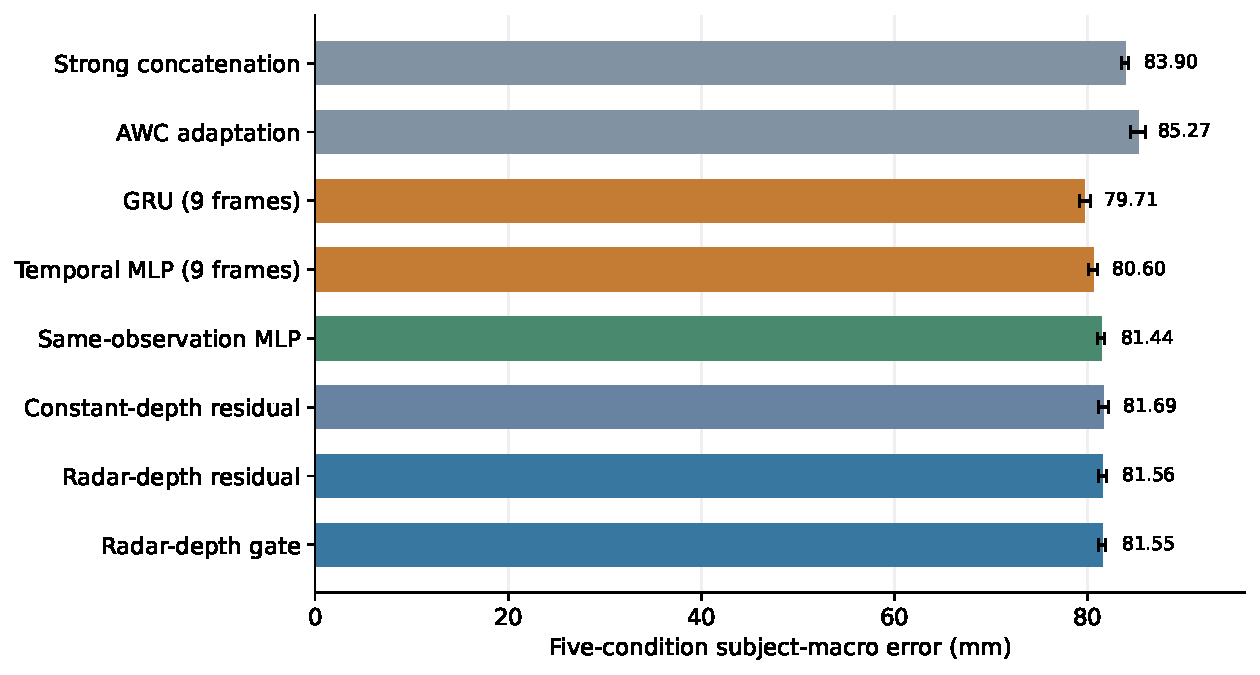
\includegraphics[width=.92\linewidth]{../figures/large_S_mm.pdf}
\caption{五条件受试者宏平均误差。时序模型具有9帧历史，几何和raw校正头为单帧。}\label{fig:largescore}
\end{figure}
\section{讨论与限制}
解释小数据几何优势为何在扩大数据后消失，区分训练预算、额外观测、表示与雷达独立作用；讨论标签来源和跨主体泛化。不要把root-relative姿态误差与其他论文全局定位误差或Human3.6M PA/N-MPJPE直接比较。
\section{结论}
待独立划分和最终协议明确后完成，不预填SOTA或创新性结论。
\bibliographystyle{plain}\bibliography{references}
\end{document}
